% $Header: /cvsroot/latex-beamer/latex-beamer/solutions/conference-talks/conference-ornate-20min.en.tex,v 1.6 2004/10/07 20:53:08 tantau Exp $

\documentclass{beamer}
%\documentclass[handout]{beamer}
%\usepackage{pgfpages}
%\pgfpagesuselayout{2 on 1}[a4paper,border shrink=5mm]

% This file is a solution template for:

% - Talk at a conference/colloquium.
% - Talk length is about 20min.
% - Style is ornate.



% Copyright 2004 by Till Tantau <tantau@users.sourceforge.net>.
%
% In principle, this file can be redistributed and/or modified under
% the terms of the GNU Public License, version 2.
%
% However, this file is supposed to be a template to be modified
% for your own needs. For this reason, if you use this file as a
% template and not specifically distribute it as part of a another
% package/program, I grant the extra permission to freely copy and
% modify this file as you see fit and even to delete this copyright
% notice.


\mode<presentation>
{
%  \usetheme{Warsaw}
%  \usetheme{Boadilla}
%  \usetheme{Goettingen}
%  \usetheme{Hannover}
%  \usetheme{Madrid}
%  \usetheme{Marburg}
%  \usetheme{Montpellier}
%  \usetheme{Pittsburgh}
  \usetheme{Hawke}
  % or ...

  \setbeamercovered{transparent}
  % or whatever (possibly just delete it)
}


\usepackage[english]{babel}
% or whatever

\usepackage[latin1]{inputenc}
% or whatever

\usepackage{times}
\usepackage[T1]{fontenc}
% Or whatever. Note that the encoding and the font should match. If T1
% does not look nice, try deleting the line with the fontenc.

\usepackage{multimedia}


%%%%%%
% My Commands
%%%%%%

\newcommand{\ml}{{\sc matlab}}
\newcommand{\bb}{{\boldsymbol{b}}}
\newcommand{\bx}{{\boldsymbol{x}}}
\newcommand{\by}{{\boldsymbol{y}}}
\newcommand{\bfm}[1]{{\boldsymbol{#1}}}

%%%%

\title[Lecture 19] % (optional, use only with long paper titles)
{Lecture 19 - Multistep Methods; accuracy, and implicit methods}

% \subtitle
% {Include Only If Paper Has a Subtitle}

\author[I. Hawke] % (optional, use only with lots of authors)
{I.~Hawke}
% - Give the names in the same order as the appear in the paper.
% - Use the \inst{?} command only if the authors have different
%   affiliation.

\institute[University of Southampton] % (optional, but mostly needed)
{
%  \inst{1}%
  School of Mathematics, \\
  University of Southampton, UK
}
% - Use the \inst command only if there are several affiliations.
% - Keep it simple, no one is interested in your street address.

\date[Semester 1] % (optional, should be abbreviation of conference name)
{MATH3018/6141, Semester 1}
% - Either use conference name or its abbreviation.
% - Not really informative to the audience, more for people (including
%   yourself) who are reading the slides online

\subject{Numerical methods}
% This is only inserted into the PDF information catalog. Can be left
% out.



% If you have a file called "university-logo-filename.xxx", where xxx
% is a graphic format that can be processed by latex or pdflatex,
% resp., then you can add a logo as follows:

\pgfdeclareimage[height=0.5cm]{university-logo}{mathematics_7469}
\logo{\pgfuseimage{university-logo}}



% Delete this, if you do not want the table of contents to pop up at
% the beginning of each subsection:
%  \AtBeginSubsection[]
%  {
%    \begin{frame}<beamer>
%      \frametitle{Outline}
%      \tableofcontents[currentsection,currentsubsection]
%    \end{frame}
%  }
\AtBeginSection[]
{
  \begin{frame}<beamer>
    \frametitle{Outline}
    \tableofcontents[currentsection]
  \end{frame}
}


% If you wish to uncover everything in a step-wise fashion, uncomment
% the following command:

%\beamerdefaultoverlayspecification{<+->}


\begin{document}

\begin{frame}
  \titlepage
\end{frame}

\section{Implicit Multistep Methods}

\subsection{Implicit Multistep Methods}

\begin{frame}
  \frametitle{Implicit Multistep Methods}

  Looking at IVPs of the form
  \begin{equation*}
    \by'(x) = \bfm{f}(x, \by(x)).
  \end{equation*}

  Looked at multistep methods using the $k$-step method formula
  \begin{equation*}
    a_k y_{n+1} + a_{k-1} y_n + \dots + a_0 y_{n+1-k} = h \left[ b_k
      f_{n+1} + b_{k-1} f_n + \dots + b_0 f_{n+1-k} \right].
  \end{equation*}
  Explicit when $b_k = 0$, as in Adams-Bashforth methods.  \pause Even
  an explicit multistep method still needs a different method to
  start; multistage methods such as Runge-Kutta are typically
  used. \pause

  \vspace{1ex}

  May want to use an \emph{implicit} formula where $b_k \neq 0$. This
  may be either for accuracy or stability, as we shall consider later.

\end{frame}


\subsection{Adams-Moulton Methods}

\begin{frame}
  \frametitle{Adams-Moulton Methods}

  \begin{overlayarea}{\textwidth}{0.9\textheight}
    \only<1->
    {
      Compare the explicit Adams-Bashforth methods
      \begin{equation*}
        y_{n+1} - y_n = h\left[ b_{k-1} f_n + b_{k-2} f_{n-1} + \dots \right]
      \end{equation*}
      with the \emph{implicit} Adams-Moulton methods
      \begin{equation*}
        y_{n+1} - y_n = h \left[ b_k f_{n+1} + b_{k-1} f_{n} + \dots \right]
      \end{equation*}
    }
    \only<2|handout:1>
    {
      As before assume the $x_j$ are evenly spaced.  Efficient as
      function evaluations can be stored, but difficult to use with
      adaptive step sizes.
    }
    \only<3-|handout:1>
    {
      Formula cannot be used directly: $f_{n+1}$ cannot be
      computed directly.
    }
    \only<4-|handout:2>
    {

      \vspace{1ex}

      Standard practice to use Adams-Moulton methods as part of a
      predictor-correct method, where estimate $y^{(p)}_{n+1}$ is
      computed, and then the unknown $f_{n+1}$ estimated as
      \begin{equation*}
        f_{n+1} = f(x_{n+1}, y^{(p)}_{n+1}).
      \end{equation*}
    }
    \only<5-|handout:2>
    {
      Typically use Adams-Bashforth as the predictor (minimizes
      function evaluations), but any method (e.g.\ RK45) valid.
    }
  \end{overlayarea}

\end{frame}

\begin{frame}
  \frametitle{Computing the coefficients}

  Computing the fixed coefficients $b_m$ is identical to
  Adams-Bashforth: integrate the formula
  \begin{equation*}
    y_{n+1} - y_n = h \left[ b_k f_{n+1} + b_{k-1} f_{n} + \dots b_1
      f_{n+2-k} \right]
  \end{equation*}
  over the range, assuming $f(x) = p_s(x)$ for polynomials of degree
  $s = 0, \dots k-1$. \pause

  \vspace{1ex}

  As before we choose as a basis for the polynomials
  \begin{equation*}
    p_s(x) = x (x + h) \dots (x + h (s-1))
  \end{equation*}
  as $p_s$ vanishes at $x = 0, -h, \dots, -h (s-1)$. \pause Then choose
  $x_{n+1} = 0, x_{n} = -h$ and so on: the resulting system of
  equations is in upper-triangular form -- solve by back substitution.

\end{frame}

\begin{frame}
  \frametitle{Adams-Moulton example}

  The Adams-Moulton method of order 5 has formula
  \begin{equation*}
    y_{n+1} - y_n = h \left[ b_5 f_{n+1} + b_4 f_{n} + b_3 f_{n-1} +
      b_2 f_{n-2} + b_1 f_{n-3} \right],
  \end{equation*} \pause
  and the coefficients follow from
  {\small
  \begin{align*}
    p_0 & = 1: & h & = h \left[ b_5 + b_4 + b_3 + b_2 + b_1 \right] \\
    p_1 & = x: & -\frac{h^2}{2} & = h \left[ -h \left( b_4 + 2 b_3 + 3
        b_2 + 4 b_1 \right) \right] \\
    p_2 & = x (x + h): & -\frac{h^3}{6} & = h \left[ h^2 \left( 2 b_3
        + 6 b_2 + 12 b_1 \right) \right] \\
    p_3 & = x (x + h) (x + 2 h): & -\frac{h^4}{4} & = h \left[ -h^3
      \left( 6 b_2 + 24 b_1 \right) \right] \\
    p_4 & = x (x + h) (x + 2 h) (x + 3 h): & -19 \frac{h^5}{30} & = h
    \left[ 24 h^4 b_1 \right].
  \end{align*}
  }
\end{frame}


\begin{frame}
  \frametitle{Standard example}

  Apply the 5 step Adams-Moulton method to
  \begin{equation*}
    y'(x) = - \sin(x), \quad y(0) = 1
  \end{equation*}
  and integrate to $x = 0.5$. Use RK4 to start algorithm and
  Adams-Bashforth 5 to predict. Using $h = 0.05$ gives
  \begin{center}
    \begin{tabular}{c|c c c c c c}
      $n$ & $x_n$ & $y_n$ & $f(x_n, y_n)$ & $\cos(x_n)$ \\
      \hline
      0 & 0.0 & 1.000 &  0.000 & 1.000 \\
      2 & 0.1 & 0.995 & -0.100 & 0.995 \\
      4 & 0.2 & 0.980 & -0.199 & 0.980 \\
      6 & 0.3 & 0.955 & -0.296 & 0.955 \\
      8 & 0.4 & 0.921 & -0.389 & 0.921 \\
      10 & 0.5 & 0.878 &        & 0.878
    \end{tabular}
  \end{center} \pause
  The error is is $2 \times 10^{-9}\%$, not visible at this precision.
  With $h = 0.01$ the error is $0.9 \times 10^{-12}\%$.  Convergence
  is slightly worse than fifth order; result is slightly biased by the
  starting method.

\end{frame}

\begin{frame}
  \frametitle{Standard Example: 2}


  Consider the system
  \begin{equation*}
    \left\{
      \begin{aligned}
        \dot{x} & = -y \\ \dot{y} & = x
      \end{aligned} \right., \quad x(0) = 1, \, \, y(0) = 0.
  \end{equation*}
  In polar coordinates this is $\dot{r} = 0$, $\dot{\phi} = 1$.
  \begin{columns}
    \begin{column}{0.5\textwidth}
      \begin{overlayarea}{\textwidth}{0.4\textheight}
        \only<2-3|handout:1>
        {
          Use Adams-Moulton 5 step method with
          $h=0.1$. At $t=500$ the result matches the correct answer to
          the eye.
        }
        \only<3|handout:1>
        {

          \vspace{1ex}
          The growth of the radius makes the errors visible.
        }
        \only<4-5|handout:2>
        {
          Use Adams-Moulton 5 step method with $h=0.01$. At $t=500$
          the result matches the correct answer to the eye.
        }
        \only<5|handout:2>
        {

          \vspace{1ex}
          Looking at the growth of the radius makes the errors
          visible even now.
        }
      \end{overlayarea}
    \end{column}
    \begin{column}{0.5\textwidth}
      \begin{overlayarea}{\textwidth}{0.6\textheight}
        \only<2|handout:0>
        {
          \begin{center}
            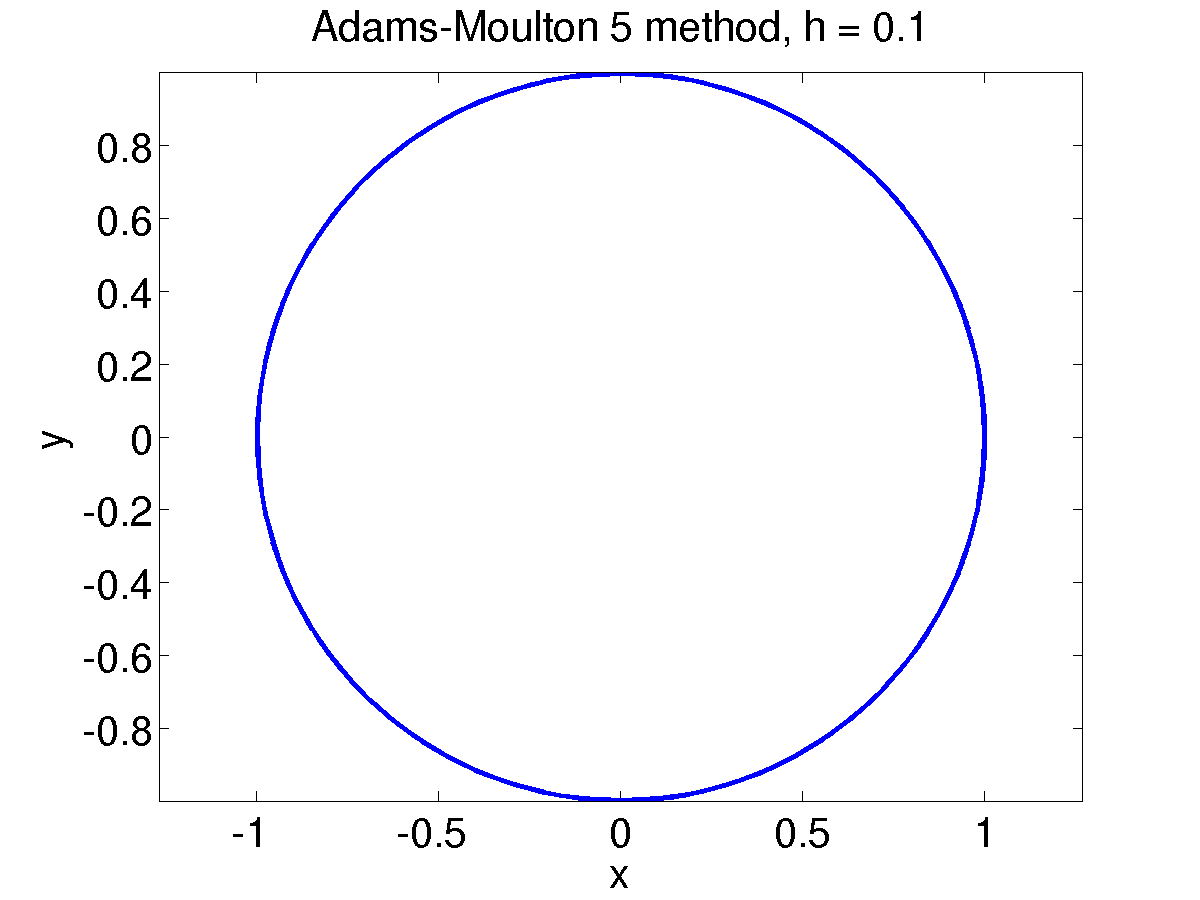
\includegraphics[height=0.5\textheight]{figures/AM5_1}
          \end{center}
        }
        \only<3|handout:1>
        {
          \begin{center}
            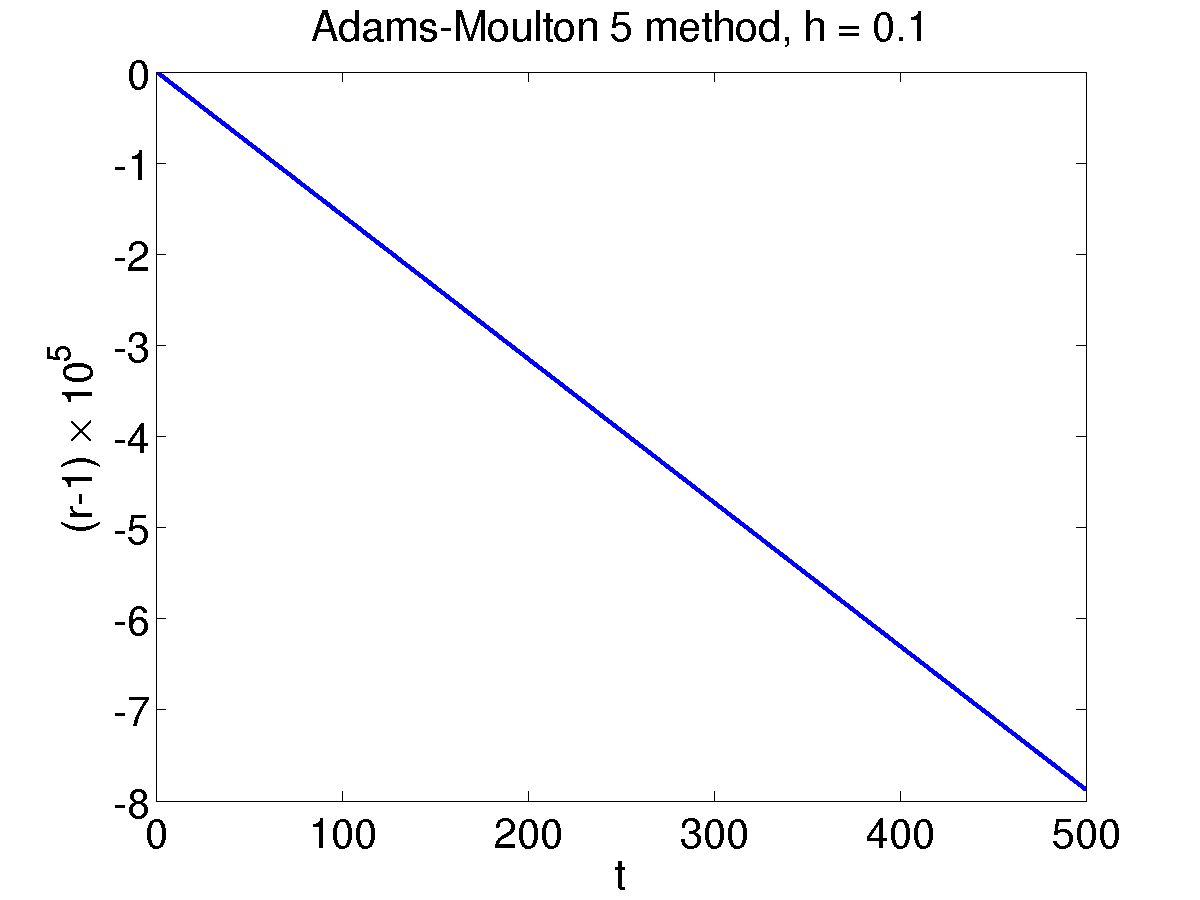
\includegraphics[height=0.5\textheight]{figures/AM5_rad1}
          \end{center}
        }
        \only<4|handout:0>
        {
          \begin{center}
            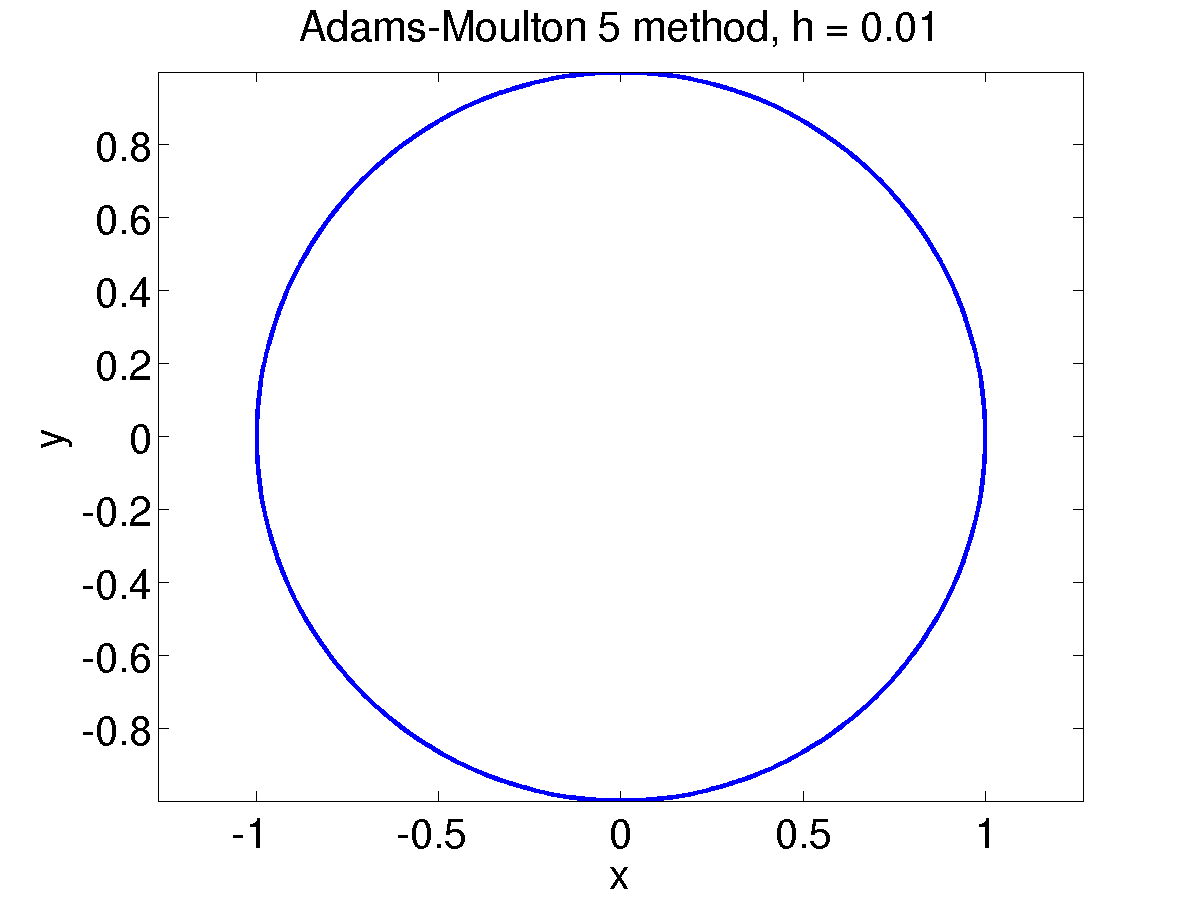
\includegraphics[height=0.5\textheight]{figures/AM5_2}
          \end{center}
        }
        \only<5|handout:2>
        {
          \begin{center}
            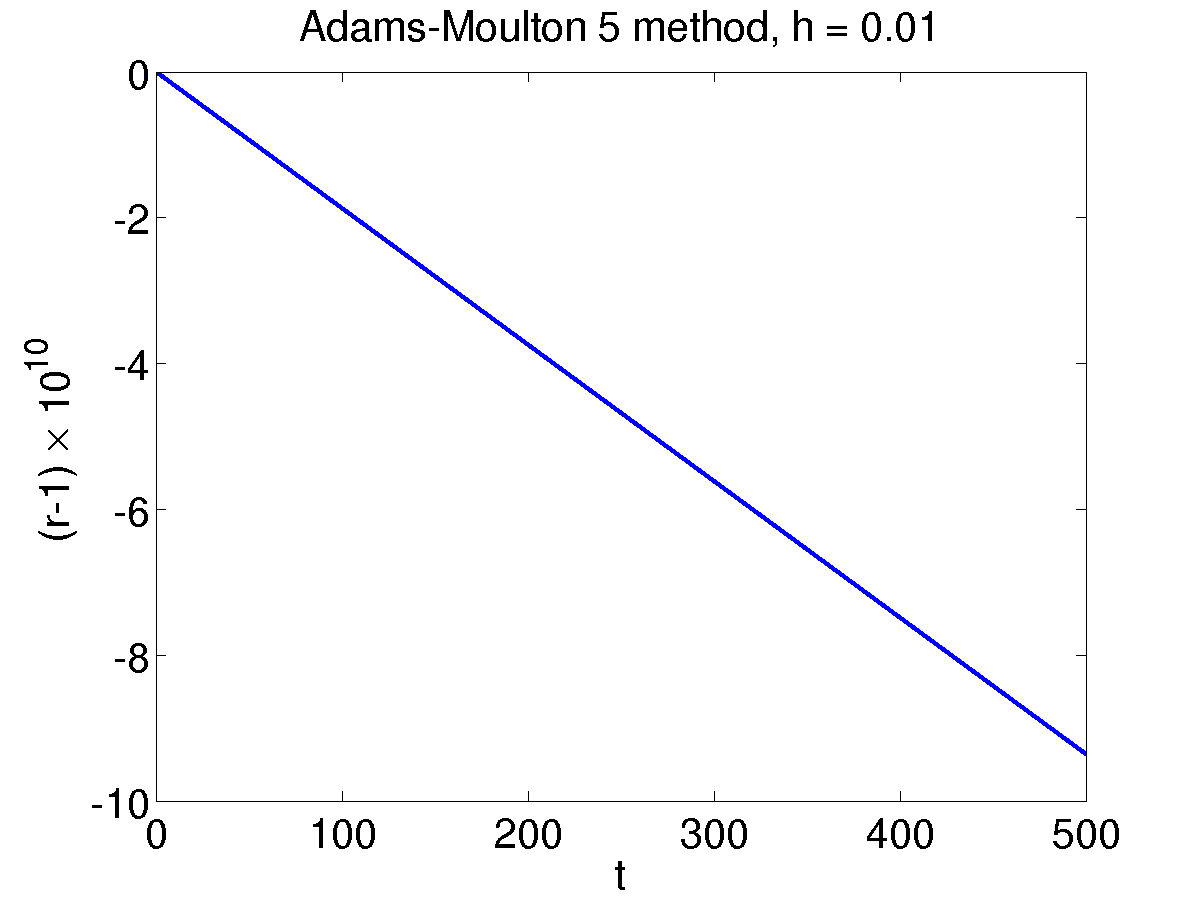
\includegraphics[height=0.5\textheight]{figures/AM5_rad2}
          \end{center}
        }
      \end{overlayarea}
    \end{column}
  \end{columns}

\end{frame}

\subsection{Order of multistep methods}

\begin{frame}
  \frametitle{Order of multistep methods}

  A $k$-step multistep method should be $k^{\text{th}}$ order accurate
  as $k^{\text{th}}$ order polynomials are exactly represented.  To
  check compute the local truncation error. \pause

  \vspace{1ex}

  For the general $k$-step method
  \begin{equation*}
    a_k y_{n+1} + a_{k-1} y_n + \dots + a_0 y_{n+1-k} = h \left[ b_k
      f_{n+1} + b_{k-1} f_n + \dots + b_0 f_{n+1-k} \right]
  \end{equation*}
  use the linear functional
  \begin{equation*}
    L(y) = \sum_{p=0}^k \left[ a_p y(x_{n-k} + p h) - h b_p y'(x_{n-k}
      + ph) \right].
  \end{equation*} \pause
  Substitute $y' = f(x, y)$ to see that the functional represents the
  $k$-step formula. Leading order term therefore gives the local
  truncation error.

\note{

Another way of thinking about the functional is the following. The
local truncation error is given by $| y_{n+1} - y(x_{n+1}) |$,
assuming that $y_n, y_{n-1}, \dots$ are all exact. We can then write
%
\begin{align*}
  \text{Error} & \propto | a_k \left( y_{n+1} - y(x_{n+1}) \right) |
  \\
  & = | -a_k y(x_{n+1}) + h \sum_{p=0}^k b_p f_{n+1-k+p} -
  \sum_{\ell=0}^{k-1} a_p y_{n+1-k+p} | \\
  \intertext{using the $k$-step formula, then}
  & = | -a_k y(x_{n+1}) + h \sum_{p=0}^k b_p y'(x_{n+1-k+p}) -
  \sum_{\ell=0}^{k-1} a_p y(x_{n+1-k+p}) | \\
  \intertext{from the IVP $y' = f$, and using that $y_n$ etc.\ are
    exact,}
  & = | \sum_{p=0}^k \left[ a_p y(x_{n-k} + p h) - h b_p y'(x_{n-k} +
    ph) \right] |
\end{align*}
%
by re-ordering the sum and shifting the location of the $x_n$ points
(which we are free to do).

}

\end{frame}

\begin{frame}
  \frametitle{Local truncation error of multistep methods}

  Take the Taylor series expansion of both $y$ and $y'$,
  \begin{equation*}
    y(x_0 + p h)  = \sum_j \frac{(p h)^j}{j!} y^{(j)}(x_0), \quad
    y'(x_0 + p h) = \sum_j \frac{(p h)^j}{j!} y^{(j+1)}(x_0),
  \end{equation*}
  and substitute in the linear functional
  \begin{equation*}
    L(y) = \sum_{p=0}^k \left[ a_p y(x_{n-k} + p h) - h b_p y'(x_{n-k}
      + ph) \right]
  \end{equation*}
  to give
  \begin{equation*}
    L(y) = d_0 y(x_0) + d_1 h y'(x_0) + d_2 h^2 y''(x_0) + \dots
  \end{equation*} \pause

  \vspace{1ex}

  Expect that the first $k$ coefficients should vanish in a
  $k$-step method.

\end{frame}

\begin{frame}
  \frametitle{Relating the coefficients}

  The $k$-step method depends on the $a_m$ and $b_m$ coefficients; the
  accuracy of the method depends on the $d_m$ coefficients. By
  matching terms in the Taylor expansion get
  \begin{align*}
    d_0 & = \sum_{p=0}^k a_p, \\
    d_1 & = \sum_{p=0}^k p a_p - b_p, \\
    d_2 & = \sum_{p=0}^k \frac{p^2}{2} a_p - p b_p,
  \end{align*} \pause
  and in general
  \begin{equation*}
    d_j = \sum_{p=0}^k \left( \frac{p^j}{j!} a_p -
      \frac{p^{j-1}}{(j-1)!} b_p \right), \quad j \geq 2.
  \end{equation*}

\end{frame}

\begin{frame}
  \frametitle{Example}

  \begin{overlayarea}{\textwidth}{0.8\textheight}
    \only<1->
    {
      For the two step Adams-Bashforth method have
    }
    \only<1-2|handout:0>
    {
      \begin{equation*}
        y_{n+1} - y_n = \frac{h}{2} \left[ 3 f_n - f_{n-1} \right].
      \end{equation*}
    }
    \only<2|handout:0>
    {
      Equivalent to the coefficients
    }
    \only<2->
    {
      \begin{equation*}
        a_2 = 1, \,\, a_1 = -1, \quad b_1 = 3/2, \,\, b_0 = -1/2.
      \end{equation*}
    }
    \only<3->
    {
      From this compute the $d_m$ coefficients:
      \begin{align*}
        d_0 & = \textstyle\sum_{p=0}^k a_p = (1 - 1) = 0, \\
        d_1 & = \textstyle\sum_{p=0}^k p a_p - b_p = \left(2 - 1
        \right) - \left( 3/2 - 1/2 \right) = 0, \\
        d_2 & = \textstyle\sum_{p=0}^k \tfrac{p^2}{2} a_p - p b_p =
        \left( 2 - 1/2 \right) - \left( 3/2 + 0 \right) = 0, \\
        d_3 & = \textstyle\sum_{p=0}^k \tfrac{p^3}{6} a_p -
        \tfrac{p^2}{2} b_p = \left( 4/3 - 1/6 \right) - \left( 1/2 \cdot
          3/2 \right) \neq 0.
      \end{align*}
    }
    \only<4->
    {
      Hence the local truncation error is ${\cal O}(h^3)$ and the
      global truncation error ${\cal O}(h^2)$.
    }
  \end{overlayarea}
\end{frame}

\begin{frame}
  \frametitle{Example: Milne's method}

  Milne's method represents $y'$ using central differencing and the
  integral with Simpson's rule:
  \begin{equation*}
    y_{n+1} - y_{n-1} = \frac{h}{3} \left( f_{n+1} + 4 f_{n} + f_{n-1} \right).
  \end{equation*} \pause
  This is a $k$-step method with coefficients
  \begin{align*}
    a_0 & = -1, & a_1 & = 0, & a_2 & = 1, \\
    b_0 & = 1/3, & b_1 & = 4/3, & b_2 & = 1/3.
  \end{align*} \pause

  \vspace{1ex}

  From this compute the accuracy coefficients
  \begin{overlayarea}{\textwidth}{0.25\textheight}
    \only<3|handout:0>
    {
      \begin{equation*}
        d_0 = a_0 + a_1 + a_2 = 0,
      \end{equation*}
    }
    \only<4|handout:0>
    {
      \begin{equation*}
        d_1 = (0 a_0 - b_0) + (a_1 - b_1) + (2 a_2 - b_2) = 0,
      \end{equation*}
    }
    \only<5|handout:0>
    {
      \begin{equation*}
        d_2 = (0 a_0 - 0 b_0) + (\frac{1}{2} a_1 - b_1) +
        (\frac{2^2}{2} a_2 - 2 b_2) = 0,
      \end{equation*}
    }
    \only<6|handout:0>
    {
      \begin{equation*}
        d_3 = (0 a_0 - 0 b_0) + (\frac{1}{6} a_1 - \frac{1}{2} b_1) +
        (\frac{2^3}{6} a_2 - \frac{2^2}{2} b_2) = 0,
      \end{equation*}
    }
    \only<7|handout:0>
    {
      \begin{equation*}
        d_4 = (0 a_0 - 0 b_0) + (\frac{1}{24} a_1 - \frac{1}{6} b_1) +
        (\frac{2^4}{24} a_2 - \frac{2^3}{6} b_2) = 0,
      \end{equation*}
    }
    \only<8->
    {
      \begin{equation*}
        d_5 = (0 a_0 - 0 b_0) + (\frac{1}{120} a_1 - \frac{1}{24} b_1) +
        (\frac{2^5}{120} a_2 - \frac{2^4}{24} b_2) \neq 0.
      \end{equation*}
    }
    \only<9>
    {
      Hence the local truncation error is $\propto h^5$ giving a
      fourth order method.
    }
  \end{overlayarea}
\end{frame}

\section{Summary}

\subsection{Summary}

\begin{frame}
  \frametitle{Summary}

  \begin{itemize}
  \item Implicit multistep methods can be used in a
    predictor-corrector fashion.
  \item Typically the implicit \emph{Adams-Moulton} methods use the
    explicit Adams-Bashforth methods as a predictor, but any explicit
    method (such as the Euler method) can be used.
  \item To check the accuracy of a general $k$-step method we Taylor
    expand the appropriate linear functional.
  \item The functional gives the error made in taking a single step;
    its local truncation error.
  \item The coefficients of the linear functional $d_m$ are given by a
    simple relation to the coefficients $a_m,b_m$ of the $k$-step
    method.
  \end{itemize}

\end{frame}

\end{document}



%%% Local Variables:
%%% mode: latex
%%% TeX-master: t
%%% End:
